\documentclass[a4paper]{jsarticle}
\usepackage[dvipdfmx]{graphicx}
\usepackage{amsmath}
\usepackage{bm}
\renewcommand{\thesection}{第\arabic{section}問}
\renewcommand{\thesubsection}{(\arabic{subsection})}
\renewcommand{\thesubsubsection}{(\alph{subsubsection})}
\begin{document}

\title{2012分野1}
\author{nakao}
\maketitle

\section{}
\subsection{}
\subsubsection{}
問題設定において$x$軸方向、$z$軸方向、回転モーメントのつりあいより、
図1のように点$B$における支点反力が得られる。
\begin{figure}[htb]
  \centering
  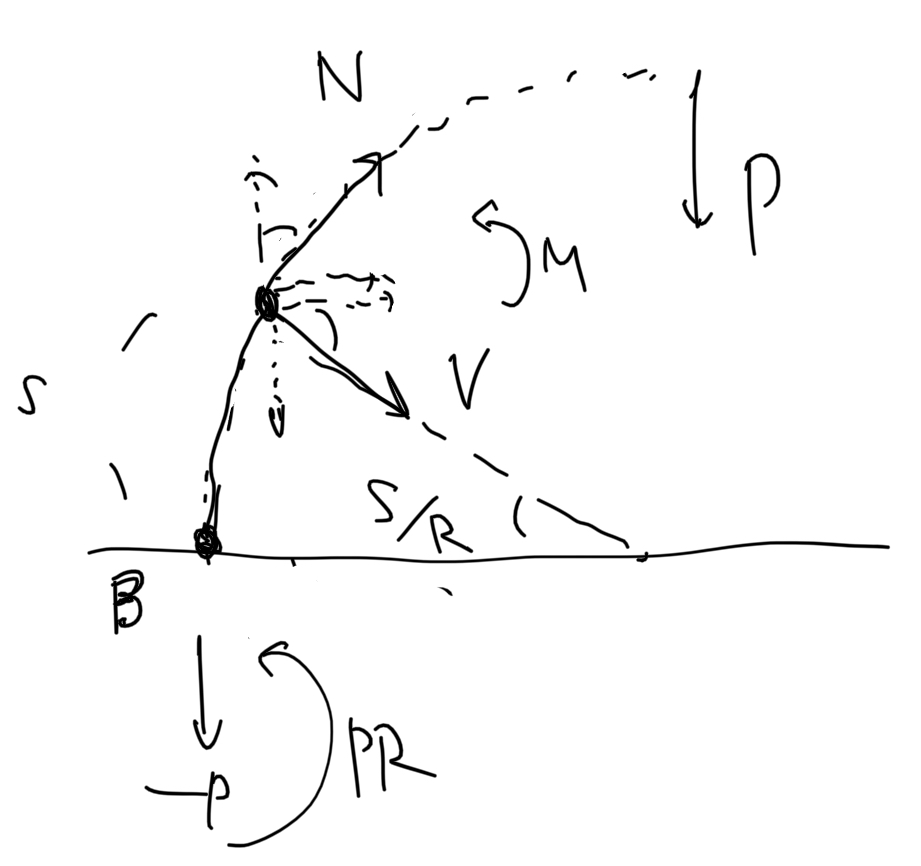
\includegraphics[width=0.3\hsize]{fig1.png}
  \caption{支点反力と内力}
\end{figure}
$s$座標が0からある$s$までの部分で力のつり合いを考えると、内力について
\begin{align}
  N \sin \frac{s}{R} + V \cos \frac{s}{R} &= 0 \\
  -N \cos \frac{s}{R} + V \sin \frac{s}{R} - P &= 0 \\
  M + P R - P R (1 - \cos \frac{s}{R}) &= 0
\end{align}
となる。これを解いて、
\begin{align}
  N &= -P \cos \frac{s}{R} \\
  V &= P \sin \frac{s}{R} \\
  M &= -P R \cos \frac{s}{R}
\end{align}
を得る。

\subsubsection{}
ベルヌーイ・オイラーの仮定より、
\begin{align}
  N &= E A \varepsilon \\
  M &= E I \lambda^{\prime}
\end{align}
が成り立つ。これより、
\begin{align}
  \varepsilon &= \frac{N}{E A} =
  -\frac{P}{E A} \cos \frac{s}{R} \\
  \lambda &= \lambda(s = 0)
  + \int_0^s \frac{M}{E I} \mathrm{d} s
  = -\frac{P R^2}{E I} \sin \frac{s}{R}
\end{align}
である。

\subsubsection{}
$s$軸に平行な方向の変位を$u_s$、垂直な方向の変位を$w_s$とする。
\begin{figure}
  \centering
  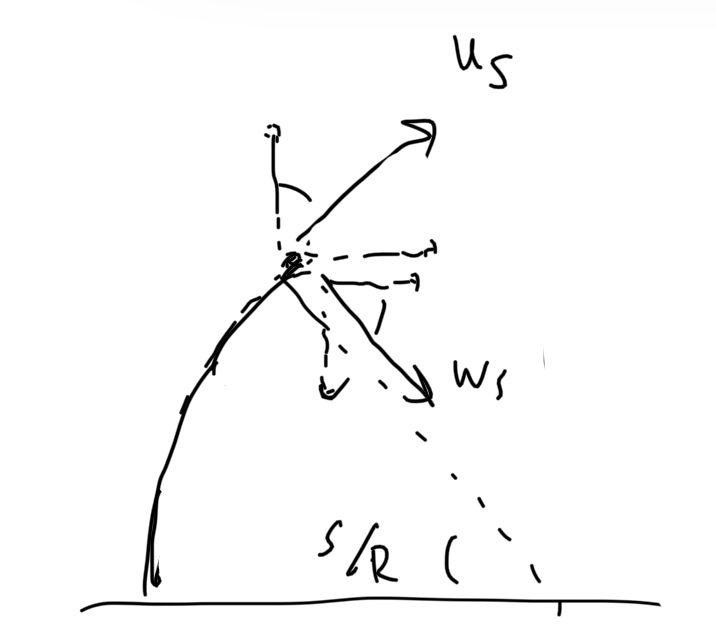
\includegraphics[width=0.3\hsize]{fig2.png}
  \caption{$u_s, w_s$の方向}
\end{figure}
$u, w, u_s, w_s$は図2のような関係にあり、
\begin{align}
  u &= u_s \sin \frac{s}{R} + w_s \cos \frac{s}{R} \\
  w &= -u_s \cos \frac{s}{R} + w_s \sin \frac{s}{R}
\end{align}
が成り立つ。式(11),(12)を$s$で微分し、
$\varepsilon = \frac{\mathrm{d} u_s}{\mathrm{d} s}, \lambda = -\frac{\mathrm{d} w_s}{\mathrm{d} s}$
を用いると、
\begin{align}
  \frac{\mathrm{d} u}{\mathrm{d} s}
  &= \varepsilon \sin \frac{s}{R} 
  - \lambda \cos \frac{s}{R} \\
  \frac{\mathrm{d} w}{\mathrm{d} s}
  &= -\varepsilon \cos \frac{s}{R} 
  - \lambda \sin \frac{s}{R}
\end{align}
であり、ここに式(9),(10)の分布を代入すると、
\begin{align}
  \frac{\mathrm{d} u}{\mathrm{d} s}
  &= -\frac{P}{E A} \cos \frac{s}{R} \sin \frac{s}{R}
  + \frac{P R^2}{E I} \cos \frac{s}{R} \sin \frac{s}{R} \\
  \frac{\mathrm{d} w}{\mathrm{d} s}
  &= \frac{P}{E A} \cos^2 \frac{s}{R} + \frac{P R^2}{E I} \sin^2 \frac{s}{R}
\end{align}
となる。

\subsubsection{}
式(15),(16)より、
\begin{align}
  u \left(s = \frac{\pi R}{2}\right) &= u(s = 0)
  + \int_0^{\frac{\pi R}{2}} \frac{\mathrm{d} u}{\mathrm{d} s} \mathrm{d} s
  = -\frac{P R}{2 E A} + \frac{P R^3}{2 E I}\\
  w \left(s = \frac{\pi R}{2}\right) &= w(s = 0)
  + \int_0^{\frac{\pi R}{2}} \frac{\mathrm{d} w}{\mathrm{d} s} \mathrm{d} s
  = \frac{\pi P R}{4 E A} + \frac{\pi P R^3}{4 E I}\\
\end{align}
を得る。

\subsection{}
$R = D/2$とする。
(1) a)と同様に支点反力を求め、内力とのつり合いを考えると、
\begin{align}
  N &= -Q \sin \frac{s}{R} \\
  V &= -Q \cos \frac{s}{R} \\
  M &= -Q R \sin \frac{s}{R}
\end{align}
を得る。ここで$s = \pi R / 2$に関する対称性より、
$\lambda(s = \pi R / 2) = 0$とすると、式(7),(8)より
\begin{align}
  \varepsilon &= \frac{N}{E A} =
  -\frac{Q}{E A} \sin \frac{s}{R} \\
  \lambda &= \lambda\left(s = \frac{\pi R}{2}\right)
  + \int_{\frac{\pi R}{2}}^s \frac{M}{E I} \mathrm{d} s
  = \frac{Q R^2}{E I} \cos \frac{s}{R}
\end{align}
となる。これらを式(13),(14)に代入すると、
\begin{align}
  \frac{\mathrm{d} u}{\mathrm{d} s}
  &= -\frac{Q}{E A} \sin^2 \frac{s}{R}
  - \frac{Q R^2}{E I} \cos^2 \frac{s}{R} \\
  \frac{\mathrm{d} w}{\mathrm{d} s}
  &= \frac{Q}{E A} \cos \frac{s}{R} \sin \frac{s}{R}
  - \frac{Q R^2}{E I} \cos \frac{s}{R} \sin \frac{s}{R}
\end{align}
を得る。したがって、
\begin{align}
  u \left(s = \frac{\pi R}{2}\right) &= u(s = 0)
  + \int_0^{\frac{\pi R}{2}} \frac{\mathrm{d} u}{\mathrm{d} s} \mathrm{d} s
  = -\frac{\pi Q R}{4 E A} - \frac{\pi Q R^3}{4 E I}\\
  w \left(s = \frac{\pi R}{2}\right) &= w(s = 0)
  + \int_0^{\frac{\pi R}{2}} \frac{\mathrm{d} w}{\mathrm{d} s} \mathrm{d} s
  = \frac{Q R}{2 E A} - \frac{Q R^3}{2 E I}
\end{align}
である。$R = D/2$を代入すると、
\begin{align}
  u \left(s = \frac{\pi R}{2}\right)
  &= -\frac{\pi Q D}{8 E A} - \frac{\pi Q D^3}{32 E I} \\
  w \left(s = \frac{\pi R}{2}\right)
  &= \frac{Q D}{4 E A} - \frac{Q D^3}{16 E I}
\end{align}
を得る。

\section{}
あーー
\end{document}